\documentclass[italian,12pt,a4paper,oneside,final]{report}
%\documentclass[italian,a4paper,titlepage]{article}
%\usepackage{amsmath}
%\usepackage{caption}
%\usepackage{subcaption}
\usepackage{graphicx}
\usepackage{biblatex} %Imports biblatex package
\usepackage[utf8]{inputenc}
\usepackage[italian]{babel}
\usepackage{csquotes}
%\usepackage[T1]{fontenc}
%\usepackage{longtable}
%\usepackage{booktabs}
%\usepackage{textcomp}
%\usepackage[draft=false]{hyperref}
%\usepackage{hyperref}
%\usepackage[table]{xcolor}
\addbibresource{iot.bib} %Import the bibliography file
\graphicspath{ {images/} }
\renewcommand{\thesection}{\arabic{section}} % remove the \chapter counter from being printed with every \section
%\hypersetup{
%	colorlinks=true,
%	linkcolor=,
%	pdftitle={Marco Giunta - Progetto IoT},
%	pdfauthor={Marco Giunta},
%}

\title{\huge Power Meter Wi-Fi con Arduino\\[0.5em]
\large Relazione Progetto IoT}
\date{Ottobre 2022}
\author{
Marco Giunta\thanks{Marco Giunta 147852 giunta.marco@spes.uniud.it}}

\begin{document}
% Generate title page
\maketitle

% Generate TOCs
\pagenumbering{arabic}
\tableofcontents

\newpage

\section{Introduzione}
Una delle sfide chiave del XXI secolo è l’adattamento ai cambiamenti climatici.
Per riuscire a limitare il riscaldamento globale, è necessario impiegare l’energia in modo efficiente, riducendo il consumo all'interno delle proprie abitazioni o negli edifici pubblici.
Per poter decidere quali misure adottare, è indispensabile conoscere il consumo reale delle apparecchiature che usiamo ogni giorno.

Con questo progetto si vuole realizzare un prototipo a basso costo di un misuratore di consumo elettrico collegato ad una rete locale tramite Wi-Fi.
Il progetto ha come obiettivo l’acquisizione e il monitoraggio dei valori di tensione, corrente e potenza presenti ai capi di un qualunque apparecchio collegato alla rete elettrica domestica (220V).
Il codice presente all'interno del dispositivo è stato progettato per permettere il collegamento contemporaneo di circa 65.000 unità, per essere in grado di monitorare, ad esempio, tutte le apparecchiature presenti all'interno di un istituto di ricerca.

Per garantire il monitoraggio di un numero così elevato di dispositivi, è stato necessario ricorrere all'utilizzo del protocollo MQTT\footfullcite{mqtt}, per ottimizzare la gestione della banda di rete e garantire l'autenticazione dei singoli dispositivi.
Per raccogliere i dati è stato utilizzato il sistema di gestione di database InfluxDB\footfullcite{influxdb} mentre, per la parte di visualizzazione tramite dashboard, è stato utilizzato il software Grafana\footfullcite{grafana}.

A solo scopo dimostrativo, il broker Mosquitto\footfullcite{mosquitto}, il collettore Telegraf\footfullcite{telegraf}, InfluxDB e Grafana sono stati configurati, utilizzando la tecnologia dei container, in una scheda single-board ARM Orange Pi PC 2 con sistema operativo Fedora IoT.

\newpage

\section{Componenti}
Per la realizzazione del prototipo sono stati utilizzati questi componenti:

\begin{itemize}
\item Arduino MKR 1000 WiFi
\item Display LCD 16×2
\item Modulo LCM1602 IIC per display LCD
\item Sensore di Corrente AC-CC da 5A con ACS712
\item Sensore di tensione con ZMPT101B
\item Divisori di tensione (da 5V a 3.3V)
\end{itemize}


\subsection{Schema elettrico}
\begin{figure}[h]
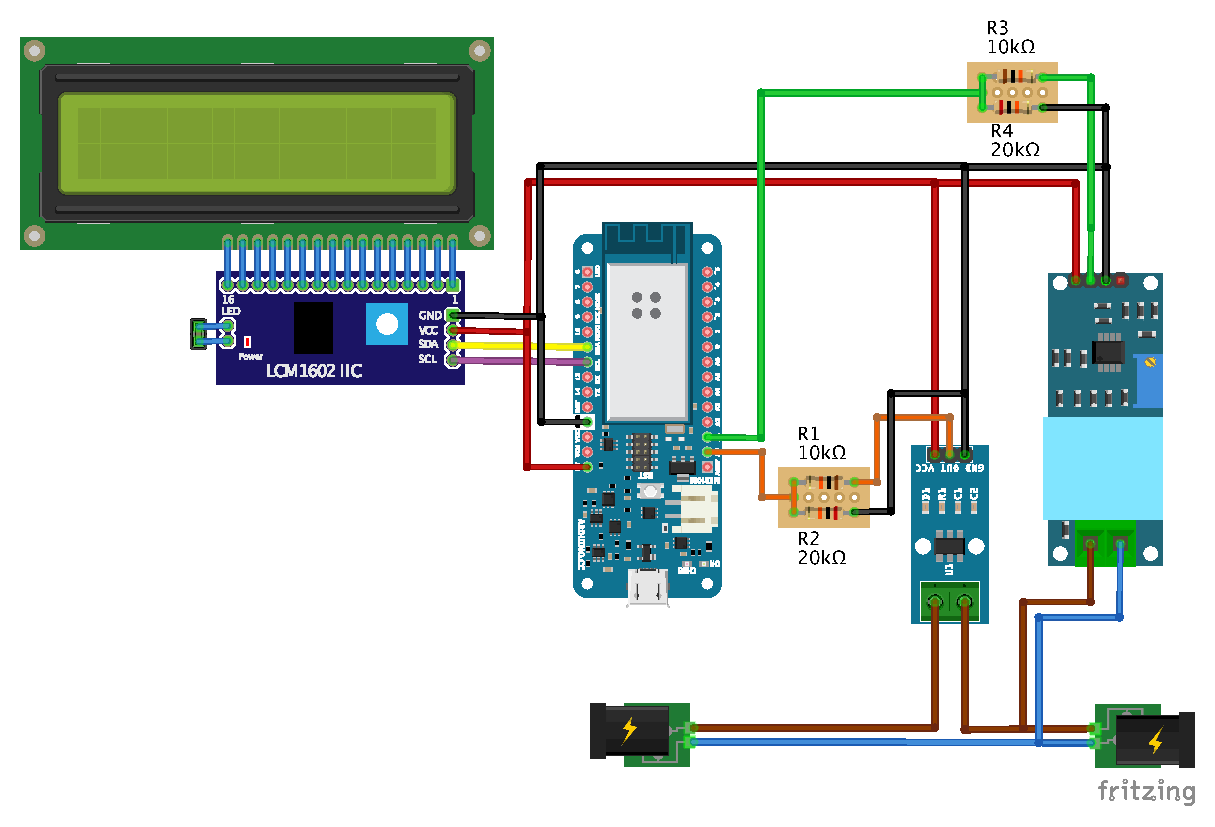
\includegraphics[width=\textwidth]{power_meter_bb.pdf}
\centering
\end{figure}

\subsection{Arduino MKR1000}
The Arduino microprocessor board is a single
board microprocessor used in intelligent projects and

prototyping. The functions performed by the
microprocessor include; sensing, controlling, logical and
computing applications. The software used in the arduino
programming is a simplified version of C/C++ language
which makes it easy to use in designing and prototyping.
The board comes in many forms such as Arduino UNO,
Arduino MEGA 2560, Arduiono Leonardo etc. It has
extensible hardware and software; it is also inexpensive
and can work across so many platforms.


Arduino has the ability to measure voltage using analog input pin. For Arduino UNO, there are 6 analog input pins (A0-A5) where you can use one of the pins to measure AC voltage. Arduino NANO has 8 pins while Arduino MEGA has 16 input pins. The analog input pins will map input voltages between 0 and 5V into integer values between 0 and 1023 with resolution of 4.9mV per unit (5.00V / 1023 units). Do not reverse the voltage polarity which may damage the pins.


\subsection{Sensore di tensione con ZMPT101B}
ZMPT101B voltage sensor module is a voltage
sensor made from the ZMPT101B voltage transformer. It
has high accuracy, good consistency for voltage and power
measurement and it can measure up to 250V AC. It is
simple to use and comes with a multi turn trim
potentiometer for adjusting the ADC output. The analysis
in this paper tends to find more accurate relationship
between the input voltage and the ADC output by
regression analysis. The ADC output is adjusted using the
trimpot to an appropriate value against a reference input.
Figure-1 is the ZMPT101B voltage sensor module.


When there is no load on output (nothing is connected to infput), the sensor has an initial voltage (Offset) of VCC/2. That is, if nothing is connected to the input and the supply voltage of the module is 5 volts, the output of the module will be 2.5 volts. 

The ZMPT101B voltage sensor module is a
voltage sensor board made from ZMPT101B potential
transformer which is capable of measuring up to 250V
AC. The sensor comes with a multi turn trim
potentiometer for adjusting the ADC output. Unlike the
current sensor where the scaling is provided by factory
trimming, the ZMPT101B sensor has to be trimmed and
calibrated by the user.


The output signal of the Single Phase AC Voltage Module is a waveform of analog values from 0 to 1023. The frequency of the wave is following the Voltage measured. Since the amplitude is adjustable, the voltage analog signal need to be calibrated. In order to calibrate, you need another voltmeter for reference. It can be either multimeter or regular voltmeter that can measure AC Voltage (RMS). The maximum voltage that the module can measured (250Vac) is referring to the Root Mean Square (RMS) value. Technically it can measure the waveform up to the peak at 353.55 Vac peak. 

The AC Voltage Module analog measurement is similar to Current Module. The voltage value will fluctuate up and down within 0 to 5V (0 to 1023 value). When no voltage detected, it will send analog signal at half the supply voltage (example 2.5V) which is about value 512. Different module will have different deviation error. Some might be reading exactly 512 when no measurement voltage detected but some may be slightly more or slightly less than value 512. You will have to manually key in the offset value during the first start or during no voltage detected. The AC Voltage Module requires at least 5V power supply and the signal output voltage is within 5V thus if you have a Arduino Nano or NodeMCU that have 3.3V analog pins, you need to add a voltage divider resistors in between to reduce or step down the output analog values.


\section{Codice}


The sensor module is a sensitive sensor. The output reading of the sensor might produce electrical noises or fake values even when there is no voltage detected. In order to greatly reduce this phenomenon, multiple samples must be taken for averaging and initial offset must be done. Our code is designed to display a value which is derived from averaging 1000 samples in a second. Each sample is recorded every 1 milli seconds (0.001 second). Each single sample value is being squared initially and once the 1000 sample values are accumulated, the average value from the 1000 samples is then being square-rooted in order to come out the Root Mean Square (RMS) voltage value which is to be displayed at Serial Monitor and LCD Display. With this averaging, the fluctuation of value is way lesser.

The second problem could be the false signal and accuracy problem. Each sensor has its own deviation error. When there is no voltage sensed, the sensor might not be 100% at middle point of voltage value. Some might be remaining at few milli voltages above / below the middle point even though after averaging. This might be due to voltage supplied not in exact 5V or due to the sensor itself. Thus 12V power adapter to power the Arduino UNO is highly recommended.

Besides, the sensor requires initial offset setting. You may need to manually offset the value by checking the false value when no voltage measurement during Arduino startup and then key in offset value in the code file. Secondly, make sure the sensor cables are tight because minor movement of wires might affects on the wire terminal connections thus affecting the accuracy reading.

Once the wave swing is calibrated to oscillate at exact middle point, after the calculation of squared, averaging and square root, there is still some minor false value existed even no voltage measurement. So our code included the second offset setting to eliminate this noise value. 



If you really read through the codes, we actually has reduced the potential wave amplitude by a factor of 0.66. 

RMSVoltageMean = (sqrt(voltageMean))*1.5;

What I realized is that by default, the waveform will start to distort before reaching 250Vac. It will affect the accuracy of other values if we calibrate based on distorted wave. So to solve this issue, I have reduced the amplitude by a factor of 0.66 in the coding, so that the waveform will not stretched till the maximum extend. You will realize when monitoring voltage is switched on, the voltage value is high and you need to reduce it. 



you can use the flash of the SAMD with the EEPROM emulation library

Microchip ATECC508A

10 Kb EEPROM Memory for Keys, Certificates, and Data


blocco di 32 bytes perchè The Read/Write command reads words (one four byte word or an 8-word block of 32 bytes)

The Write command writes either one four byte word or an 8-word block of 32 bytes to one of the
EEPROM zones on the device.

I would use a union because then the data exists in two different formats at the same time without any need for conversion.

slot 8 Typical Use Data Bytes 416


\subsection{Potenza reale e apparente}
Apparent power is the product of the root mean square(rms) values of the current and voltage

Real power is the product of the instantaneous values of the current and voltage in the circuit

The unit of Apparent power is Volt Ampere(VA)


The unit of Real Power is Watt



\end{document}
